\chapter{Exercise Solutions}

\section{1. Science skills}

\subsection{Exercise 1-1} 
\begin{multicols}{4}
\begin{enumerate}[noitemsep, label=\textbf{\arabic*}. ] 
\item %Carry out the following calculations
  \begin{enumerate}[itemsep=5pt, label=\textbf{(\alph*)} ] 
    \item $3,63 \times 10^6$
    \item $37,83$
    \item $6,3 \times 10^{−4}$
    \end{enumerate}
\item %Write the following in scientific notation using Table 1.3 as a reference.
    \begin{enumerate}[itemsep=5pt, label=\textbf{(\alph*)} ] 
    \item $5,11 \times 10^{5} \text{ V}$
    \item $1,0 \times 10^{-1} \ell$
    \item $5 \times 10^{-7} \text{ m}$
    \item $2,50 \times 10^{-7} \text{ m}$
    \item $3,5 \times 10^{-2} \text{ g}$
    \end{enumerate}
 \item %Write the following using the prefixes in Table 1.3.
    \begin{enumerate}[itemsep=5pt, label=\textbf{(\alph*)} ] 
    \item $0,1602 \text{ aC}$
    \item $1,992 \text{ MJ}$
    \item $59,8 \text{ kN}$
    \item $2,5 \text{ mA}$
    \item $7,5 \text{ km}$
    \end{enumerate}
\end{enumerate}
\end{multicols}
\subsection{Exercise 1-2} 
\begin{multicols}{3}
\begin{enumerate}[itemsep=5pt, label=\textbf{\arabic*}. ]
\item %Write the following quantities in scientific notation
    \begin{enumerate}[itemsep=5pt, label=\textbf{(\alph*)} ] 
    \item $1,01 \times 10^{4} \text{ Pa}$
    \item $9,8 \times 10^2 \text{ m} \cdot \text{s}^{−2}$
    \item $1,256 \times 10^{−6} \text{ A}$
    \end{enumerate}
\item %For each of the following symbols, write out the unit in full and write what power of 10 it represents:
    \begin{enumerate}[itemsep=5pt, label=\textbf{(\alph*)} ] 
    \item microgram and $-6$
    \item milligram and $-3$
    \item kilogram and $3$
    \item megagram and $6$
    \end{enumerate}
\item %Write each of the following in scientific notation, correct to 2 decimal places:
    \begin{enumerate}[itemsep=5pt, label=\textbf{(\alph*)} ] 
    \item $1,23 \times 10^{−6} \text{ N}$
    \item $4,17 \times 10^8 \text{ kg}$
    \item $2,47 \times 10^5 \text{ A}$
    \item $8,80 \times 10^{−4} \text{ mm}$
    \end{enumerate}
\item %For each of the following, write the measurement using the correct symbol for the prefix and the base unit:
    \begin{enumerate}[itemsep=5pt, label=\textbf{(\alph*)} ] 
    \item $1,01 \mu \text{s}$
    \item $1~000 \text{ mg}$
    \item $7,2 \text{ Mm}$
    \item $11 \text{ n} \ell $
    \end{enumerate}
\item % the concorde
$234,44 \text{ m} \cdot \text{ s}^{−1}$
\item % water bp
$373 \text{ K}$
\end{enumerate}
\end{multicols}

\section {2. Classification of matter}
% \subsection{Exercise 2-1} %p. 50-51 This is a table to be completed

\subsection{Exercise 2-2} 
\begin{multicols}{3}
\begin{enumerate}[itemsep=5pt, label=\textbf{\arabic*}. ] 
\item % fill in table
  \begin{enumerate}
   \item heterogeneous mixture
   \item homogeneous mixture
   \item pure
   \item pure
   \item heterogeneous mixture
   \item homogeneous mixture
  \end{enumerate}
\item % In each of the following cases, say whether the substance is an element, a mixture or a compound. 
  \begin{enumerate}
   \item element
   \item mixture
   \item element
   \item compound
   \item compound
  \end{enumerate}         
\end{enumerate}
\end{multicols}

\subsection{Exercise 2-3} 
\begin{multicols}{3}
\begin{enumerate}[noitemsep, label=\textbf{\arabic*}. ] 
\item %formula for calcium carbonate 
\begin{enumerate}[noitemsep, label=\textbf{(\alph*)} ] 
\item compound
\item $1:1:3$
\end{enumerate}
\item %give the name of the following substances
\begin{enumerate}[noitemsep, label=\textbf{(\alph*)} ] 
\item Potassium bromide
\item Hydrochloric acid
\item Potassium permanganate
\item Nitrogen dioxide
\item Ammonium hydroxide
\item Sodium sulphate
\item Iron (III) nitrate
\item Lead (II) sulphite
\item Copper (II) hydrogen carbonate
\end{enumerate}
\item %Give the chemical formula
\begin{enumerate}[noitemsep, label=\textbf{(\alph*)} ] 
\item $\text{KNO}_3$
\item $\text{Na}_{2}\text{O}$
\item $\text{BaSO}_4$
\item $\text{AlCl}_3$
\item $\text{Mg}_{3}\text{(PO}_4\text{)}_{2}$
\item $\text{SnBr}_2$
\item $\text{Mn}_{3}\text{P}_{2}$
\end{enumerate}
\end{enumerate}
\end{multicols}

\subsection{End of chapter exercises} 
\begin{multicols}{3} 
\begin{enumerate}[itemsep=5pt, label=\textbf{\arabic*}. ] 
 \item %MCQ
\begin{enumerate}[itemsep=6pt,label=\textbf{(\alph*)}]
\item i
\item iii
\end{enumerate}
\item %Classify each of the following
\begin{enumerate}[itemsep=6pt,label=\textbf{(\alph*)}]
\item compound
\item compound
\item heterogeneous mixture
\item solution
\item solution
\item compound
\item element
\item solution
\end{enumerate}
\item %match columns
\begin{enumerate}[itemsep=5pt,label=\textbf{(\alph*)}]
\item D  
\item A
\item E
\item B
\item C
\end{enumerate}
\item %testtube with iron and sulphur
\begin{enumerate}[itemsep=5pt,label=\textbf{(\alph*)}]
\item use a magnet
\item magnetism
\end{enumerate}
\item %given descriptions
\begin{enumerate}[itemsep=5pt,label=\textbf{(\alph*)}]
 \item $\text{Ag}$
 \item $\text{KBr}$
 \item $\text{CO}_{2}$
\end{enumerate}
\item %give names
\begin{enumerate}[itemsep=5pt,label=\textbf{(\alph*)}]
 \item sodium bromide
 \item barium sulphate
 \item sulphur dioxide
 \item sulphuric acid
\end{enumerate}
\item %give formula
\begin{enumerate}[itemsep=5pt,label=\textbf{(\alph*)}]
 \item $\text{FeSO}_{4}$
 \item $\text{BF}_{3}$
 \item $\text{KMnO}_{4}$
 \item $\text{ZnCl}_{2}$
\end{enumerate}
\item %properties
\begin{enumerate}[itemsep=5pt,label=\textbf{(\alph*)}]
 \item friction
 \item durable
 \item durable
 \item shiny
 \item easily moulded
 \item fibrous
\end{enumerate}
\end{enumerate}
\end{multicols}

\section {3. States of matter and the KMT}
\subsection{End of chapter exercises} 
\begin{multicols}{3}
\begin{enumerate}[label=\textbf{\arabic*}., itemsep=5pt]
\item %give one word/term
\begin{enumerate}[label=\textbf{(\alph*)}, itemsep=7pt]
\item sublimation
\item evaporation
\end{enumerate}
\item %water
\begin{enumerate}[label=\textbf{(\alph*)}, itemsep=7pt]
\item see definition
\item liquid to gas
\end{enumerate}
\item %describe a solid
see definition
\item %table
\begin{enumerate}
 \item solid, solid, gas, solid, gas, solid
\item carbon 
\item helium
\end{enumerate}
\item %pics
\scalebox{.3}{
\begin{pspicture}(0,0)(10,2.6)
\SpecialCoor
%\psgrid[gridcolor=lightgray]

\rput(0,0.5){\psframe(0,0)(3,2)
\rput(0.1,0){\multirput(0.2,0.2)(0.4,0){7}{\pscircle(0,0){0.2}}
\multirput(0.4,0.55)(0.4,0){6}{\pscircle(0,0){0.2}}
\multirput(0.2,0.9)(0.4,0){7}{\pscircle(0,0){0.2}}}}

\rput(3.5,0.5){\psframe(0,0)(3,2)
\rput(0.2,0.2){\pscircle(0,0){0.2}}
\rput(0.6,0.3){\pscircle(0,0){0.2}}
\rput(1.2,0.3){\pscircle(0,0){0.2}}
\rput(1.7,0.2){\pscircle(0,0){0.2}}
\rput(2.3,0.3){\pscircle(0,0){0.2}}
\rput(2.8,0.2){\pscircle(0,0){0.2}}
\rput(0.3,0.9){\pscircle(0,0){0.2}}
\rput(0.8,0.7){\pscircle(0,0){0.2}}
\rput(1.5,0.8){\pscircle(0,0){0.2}}
\rput(2.0,0.8){\pscircle(0,0){0.2}}
\rput(2.5,0.7){\pscircle(0,0){0.2}}}

\rput(7,0.5){\psframe(0,0)(3,2)
\rput(2.5,0.5){\pscircle(0,0){0.2}}
\rput(2.4,1.7){\pscircle(0,0){0.2}}
\rput(1.5,1){\pscircle(0,0){0.2}}
\rput(0.7,1.7){\pscircle(0,0){0.2}}
\rput(0.3,0.3){\pscircle(0,0){0.2}}}

\uput[d](1.5,0.5){solid}
\uput[d](5,0.5){liquid}
\uput[d](8.5,0.5){gas}

\end{pspicture}}
\end{enumerate}
\end{multicols}


% \end{eocexercises}

\section {4. The atom}
\subsection{Exercise 4-1} 
\begin{multicols}{5}
\begin{enumerate}[noitemsep, label=\textbf{\arabic*}. ] 
\item D
\item A
\item C
\item E
\item B
\end{enumerate}
\end{multicols}
\subsection{Exercise 4-2}
\begin{multicols}{5}
\begin{enumerate}[noitemsep, label=\textbf{\arabic*}. ]
 \item %explain meaning
see definitions
\end{enumerate}
%  \item table
\begin{enumerate}[noitemsep, label=\textbf{\arabic*}. ]
\setcounter{enumi}{2}
 \item %standard notation
\begin{enumerate}[noitemsep, label=\textbf{\alph*}. ]
 \item $^{40}_{19}\text{K}$
\item $^{54}_{29}\text{Cu}$
\item $^{35}_{17}\text{Cl}$
\end{enumerate}
 \item %for the element
\begin{enumerate}[noitemsep, label=\textbf{\alph*}. ]
 \item $17$
\item $18$
\item $17$
\end{enumerate}
 \item %which of the following atoms
$^{15}_{7}\text{N}$
 \item %give x
\begin{enumerate}[noitemsep, label=\textbf{\alph*}. ]
 \item Ar
\item $40$
\item $15$
\end{enumerate}
 \item %complete table
\begin{enumerate}[noitemsep, label=\textbf{\alph*}. ]
 \item $Z$
\item $N, A$
\end{enumerate}
\end{enumerate}
\end{multicols}
\subsection{Exercise 4-3}
\begin{multicols}{5}
\begin{enumerate}[noitemsep, label=\textbf{\arabic*}. ]
 \item %MCQ
D
 \item %sulphur isotopes
\begin{enumerate}[noitemsep, label=\textbf{\alph*}. ]
 \item $16$
\item $32$ and $34$
\item $16$
\item $16$ and $18$
\end{enumerate}
 \item %MCQ
C
 \item %MCQ
A
\end{enumerate}
\begin{enumerate}[noitemsep, label=\textbf{\arabic*}. ]
\setcounter{enumi}{5}
 \item %boron
$10,8 \text{ u}$
 \item %magnesium
$24,3 \text{ u}$
\item %std notation
\begin{enumerate}[noitemsep, label=\textbf{\alph*}. ]
 \item $^{232}_{92}\text{U}$
\item $^{238}_{92}\text{U}$
\end{enumerate}
\item %MCQ
B
\item %sulphur isotopes
\begin{enumerate}[noitemsep, label=\textbf{\alph*}. ]
 \item $16$
\item  $33$
\item $16$
\item $17$
\end{enumerate}
\end{enumerate}
\end{multicols}
\subsection{End of chapter exercises} 
\begin{multicols}{4}
\begin{enumerate}[noitemsep, label=\textbf{\arabic*}. ] 
\item %give word
    \begin{enumerate}[noitemsep, label=\textbf{(\alph*)} ]
    \item atomic mass number
    \item electron orbital
    \end{enumerate}
\item %true/false
    \begin{enumerate}[noitemsep, label=\textbf{(\alph*)} ]
    \item false
    \item true
    \item true
    \item false
    \end{enumerate}
\item %MCQ
    \begin{enumerate}[noitemsep, label=\textbf{(\alph*)} ]
    \item B
    \item B
    \item A
    \item C
    \item B
    \end{enumerate}
\item %give std notation
    \begin{enumerate}[noitemsep, label=\textbf{(\alph*)} ]
    \item $^{5}_{4}\text{Be}$
    \item $^{12}_{6}\text{C}$
    \item $^{48}_{22}\text{Ti}$
    \item $^{19}_{9}\text{F}$
    \end{enumerate}
\item %electron configs
    \begin{enumerate}[noitemsep, label=\textbf{(\alph*)} ]
    \item $\text{[Ne]} 3\text{s}^2 3\text{p}^1$
    \item $\text{[Ne]} 3\text{s}^2 3\text{p}^3$
    \item $\text{[He]} 2\text{s}^2 2\text{p}^2$
    \item $\text{[He]} 2\text{s}^2 2\text{p}^6$
    \item $\text{[Ne]} 3\text{s}^2 3\text{p}^6$
    \end{enumerate}
\item %give protons,etc.
    \begin{enumerate}[noitemsep, label=\textbf{(\alph*)} ]
    \item $78 ; 117 ; 78$
    \item $18 ; 22 ; 18$
    \item $27 ; 32 ; 27$
    \item $3 ; 4 ; 3$
    \item $5 ; 6 ; 5$
    \end{enumerate}
\item %give x
  \begin{enumerate}[noitemsep, label=\textbf{(\alph*)} ]
  \item Rh
  \item $17$
  \item $9$
  \end{enumerate}
\item %isotopes
B
\item %copper amu
$63,62 \text{ u}$
\end{enumerate}
\end{multicols}
\section {5. The periodic table}
\subsection{Exercise 5-2} 
\begin{multicols}{5}
\begin{enumerate}[noitemsep, label=\textbf{\arabic*}. ] 
\setcounter{3}
\item %elements list
    \begin{enumerate}[noitemsep, label=\textbf{(\alph*)} ]  
    \item Li
\item Cl
\item Ne
\item Li
\item C
\item Li
\item Ca
\item Ne
\item Mg and Ca
    \end{enumerate}  
\end{enumerate}
\end{multicols}
\subsection{End of chapter exercises} 
\begin{multicols}{3}
    \begin{enumerate}[itemsep=6pt, label=\textbf{\arabic*}. ] 
\item %true false 
 \begin{enumerate}[noitemsep, label=\textbf{(\alph*)} ]
    \item false
    \item true
    \item false
    \item false
    \end{enumerate}
\item %one word/term 
 \begin{enumerate}[noitemsep, label=\textbf{(\alph*)} ]
    \item first ionisation energy
    \item period
    \item halogens
    \end{enumerate}
\item %compare elements 
 \begin{enumerate}[noitemsep, label=\textbf{(\alph*)} ] 
    \item $\text{Br} > \text{ Cl}$
    \item $\text{Cl} > \text{ Br}$ 
    \item $\text{Cl} > \text{ Br}$
    \item $\text{Br} > \text{ Cl}$
    \end{enumerate}
\item %draw graphs 
 \begin{enumerate}[noitemsep, label=\textbf{(\alph*)} ]
    \item \includegraphics[width=.2\textwidth]{photos/periodictable_eocex_graph1.png}
    \item \includegraphics[width=.2\textwidth]{photos/periodictable_eocex_graph2.png}
    \item 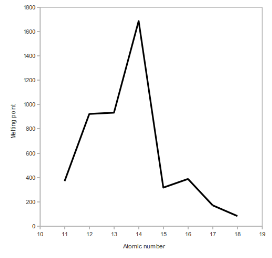
\includegraphics[width=.2\textwidth]{photos/periodictable_eocex_graph3.png}
    \item \includegraphics[width=.2\textwidth]{photos/periodic_table_eocex_graph4.png}
    \end{enumerate}
\end{enumerate}
\end{multicols}

\section {6. Chemical bonding}
\subsection{Exercise 6-1} 
    \begin{enumerate}[noitemsep, label=\textbf{\arabic*}.]
	\item %An amount of R~$3~500$ is invested in a savings account which pays simple interest at a rate of $7,5\%$ per annum. Calculate the balance accumulated by the end of 2 years.

	\item %Calculate the accumulated amount in the following situations:
	\begin{enumerate}[noitemsep, label=\textbf{(\alph*)} ]
	    \item %A loan of R~$300$ at a rate of $8\%$ for 1 year.

	    \item %An investment of R~$2~250$ at a rate of $12,5\%$p.a. for 6 years.
	\end{enumerate}

	\item %Sally wanted to calculate the number of years she needed to invest R~$1~000$ for in order to accumulate R~$2~500$. She has been offered a simple interest rate of $8,2\%$ p.a. How many years will it take for the money to grow to R~$2~500$?

	\item %Joseph made a deposit of R~$5~000$ in the bank for his 5 year old son’s 21st birthday. He has given his son the amount of R~$18~000$ on his birthday. At what rate was the money invested, if simple interest was calculated?\\
    \end{enumerate}

% }
% \end{exercises}
\subsection{Exercise 6-2} %p. 197
% \begin{exercises}{}{
    \begin{enumerate}[label=\textbf{\arabic*}.]
	\item %Vanessa wants to buy a fridge on a hire purchase agreement. The cash price of the fridge is R~$4~500$. She is required to pay a deposit of $15\%$ and pay the remaining loan amount off over 24 months at an interest rate of $12\%$ p.a.
	\begin{enumerate}[noitemsep, label=\textbf{(\alph*)} ]
	    \item %What is the principal loan amount?
	    \item %What is the accumulated loan amount?
	    \item %What are Vanessa’s monthly repayments?
	    \item %What is the total amount she has paid for the fridge?
	\end{enumerate}


	\item %Bongani buys a dining room table costing R~$8~500$ on a hire purchase agreement. He is charged an interest rate of $17,5\%$p.a. over 3 years.
	\begin{enumerate}[noitemsep, label=\textbf{(\alph*)} ]
	    \item %How much will Bongani pay in total?
	    \item %How much interest does he pay?
	    \item %What is his monthly instalment?
	\end{enumerate}

	\item %A lounge suite is advertised on TV, to be paid off over 36 months at R~$150$ a month.
	\begin{enumerate}[noitemsep, label=\textbf{(\alph*)} ]
	    \item %Assuming that no deposit is needed, how much will the buyer pay for the lounge suite once it has been paid off?
	    \item %If the interest rate is $9\%$ p.a, what is the cash price of the suite?\\
	\end{enumerate}
    \end{enumerate}
% }
% \end{exercises}
\subsection{Exercise 6-3} %p. 204
% \begin{exercises}{}{
    \begin{enumerate}[label=\textbf{\arabic*}.]
	\item %An amount of R~$3~500$ is invested in a savings account which pays a compound interest rate of $7,5\%$ p.a. Calculate the balance accumulated by the end of 2 years.

	\item %Morgan invests R~$5~000$ into an account which pays out a lump sum at the end of 5 years. If he gets R~$7~500$ at the end of the period, what compound interest rate did the bank offer him?

	\item %Nicola wants to invest some money at a compound interest rate of $11\%$ p.a. How much money (to the nearest Rand) should be invested if she wants to reach a sum of R~$100~000$ in five years time?\\
    \end{enumerate}

% }
% \end{exercises}
\subsection{Exercise 6-4} %p.207
% \begin{exercises}{}{
    \begin{enumerate}[label=\textbf{\arabic*}.]
	\item %If the average rate of inflation for the past few years was $7,3\%$ p.a. and your water and electricity account is R~$1~425$ on average, what would you expect to pay in 6 years time?

	\item %The price of popcorn and a coke at the movies is now R~$60$. If the average rate of inflation is $9,2\%$ p.a., what was the price of popcorn and coke 5 years ago?

	\item %A small town in Ohio, USA is experience a huge increase in births. If the average growth rate of the population is $16\%$ p.a, how many babies will be born to the 1600 residents in the next 2 years?\\
    \end{enumerate}

% }
% \end{exercises}
\subsection{Exercise 6-5} %p.209
% \begin{exercises}{}
% {
    \begin{enumerate}[itemsep=6pt, label=\textbf{\arabic*}.]
	\item %Bridget wants to buy an iPod that costs £~$100$, with the exchange rate currently at £~$1$ $=$ R~$14$. She estimates that the exchange rate will drop to R~$12$ in a month.
	\begin{enumerate}[noitemsep, label=\textbf{(\alph*)} ]
	    \item %How much will the MP3 player cost in Rands, if she buys it now?
	    \item %How much will she save if the exchange rate drops to R~$12$?
	    \item %How much will she lose if the exchange rate moves to R~$15$?
	\end{enumerate}

	\item %Study the following exchange rate table:\\
	
	\begin{enumerate}[noitemsep, label=\textbf{(\alph*)} ]
	    \item %In South Africa the cost of a new Honda Civic is R~$173~400$. In England the same vehicle costs £~$12~200$ and in the USA \$~$21~900$. In which country is the car the cheapest?

	    \item %Sollie and Arinda are waiters in a South African restaurant attracting many tourists from abroad. Sollie gets a £~$6$ tip from a tourist and Arinda gets \$~$12$. Who got the better tip?
	\end{enumerate}
    \end{enumerate}

% }
% \end{exercises}

\subsection{End of chapter exercises} %p.210-211
% \begin{eocexercises}{}
    \begin{enumerate}[label=\textbf{\arabic*}.]
	\item %Alison is going on holiday to Europe. Her hotel will cost €~$200$ per night. How much will she need in Rands to cover her hotel bill, if the exchange rate is €~$1$ = R~$9,20$?

	\item %Calculate how much you will earn if you invested R~$500$ for 1 year at the following interest rates:
	\begin{enumerate}[noitemsep, label=\textbf{(\alph*)} ]
	    \item %$6,85\%$ simple interest
	    \item %$4,00\%$ compound interest
	\end{enumerate}

	\item %Bianca has R~$1~450$ to invest for 3 years. Bank A offers a savings account which pays simple interest at a rate of $11\%$ per annum, whereas Bank B offers a savings account paying compound interest at a rate of $10,5\%$ per annum. Which account would leave Bianca with the highest accumulated balance at the end of the 3 year period?

	\item %How much simple interest is payable on a loan of R~$2~000$ for a year, if the interest rate is $10\%$ p.a.?

	\item %How much compound interest is payable on a loan of R~$2~000$ for a year, if the interest rate is $10\%$ p.a.?

	\item %Discuss:
	\begin{enumerate}[noitemsep, label=\textbf{(\alph*)} ]
	    \item %Which type of interest would you like to use if you are the borrower?

	    \item %Which type of interest would you like to use if you were the banker?
	\end{enumerate}

	\item %Calculate the compound interest for the following problems.
	\begin{enumerate}[noitemsep, label=\textbf{(\alph*)} ]
	    \item %A R~$2~000$ loan for 2 years at $5\%$ p.a..
	    \item %A R~$1~500$ investment for 3 years at $6\%$ p.a..
	    \item %A R~$800$ loan for 1 year at $16\%$ p.a..
	\end{enumerate}

	\item %If the exchange rate for ¥~$100$ = R~$6,2287$ (¥ = Yen) and 1 Australian Dollar (AUD) = R~$5,1094$, determine the exchange rate between the Australian Dollar and the Japanese Yen.

	\item %Bonnie bought a stove for R~$3~750$. After 3 years she had finished paying for it and the R~$956,25$ interest that was charged for hire purchase. Determine the rate of simple interest that was charged.
    \end{enumerate}

% \end{eocexercises}

\section {7. Transverse pulses}
\subsection{Exercise 7-1} %p. 218-219
% \begin{exercises}{}
% {
\begin{enumerate}[itemsep=5pt, label=\textbf{\arabic*}. ]
\item %In each of the following triangles, state whether $a$, $b$ and $c$ are the hypotenuse, opposite or adjacent sides of the triangle with respect to $\theta$. 
% \setcounter{subfigure}{0}
\begin{enumerate}[noitemsep, label=\textbf{(\alph*)} ]
 \item 
\item 
\item 
\item 
\item 
\item 
\end{enumerate}



\item %Use your calculator to determine the value of the following (correct to $2$ decimal places):
\begin{enumerate}[noitemsep, label=\textbf{(\alph*)} ]
\begin{multicols}{2} 
% \setcounter{enumi}{6} 
\item %$tan~65^{\circ}$
\item %$sin~38^{\circ}$
\item %$cos~74^{\circ}$
\item %$sin~12^{\circ}$
\item %$cos~26^{\circ}$
\item %$tan~49^{\circ}$
\item %$\frac{1}{4}~cos~20^{\circ}$
\item %$3~tan~40^{\circ}$
\item %$\frac{2}{3}~sin~90^{\circ}$
\end{multicols}
\end{enumerate}

\item %If $x=39^{\circ}$ and $y=21^{\circ}$ use a calculator to determine whether the following statements are true or false:
\begin{enumerate}[noitemsep, label=\textbf{(\alph*)} ]
\begin{multicols}{2} 
% \setcounter{enumi}{15} 
\item %$cos~x + 2~cos~x=3~cos~x$
\item %$cos~2y = cos~y+cos~y$
\item %$tan~x=\dfrac{sin~x}{cos~x}$
\item %$cos~(x+y) = cos~x+cos~y$
\end{multicols}
\end{enumerate}


\item %Complete each of the following (the first example has been done):



\begin{enumerate}[noitemsep, label=\textbf{(\alph*)} ]
\begin{multicols}{2}
% \setcounter{enumi}{19}
\item %$sin~\hat{A} = \frac{\mbox{opposite}}{\mbox{hypotenuse}}=\dfrac{CB}{AC}$
\item %$cos~\hat{A} = $
\item %$tan~\hat{A}= $
\item %$sin~\hat{C}= $
\item %$cos~\hat{C}= $
\item %$tan~\hat{C}= $
\end{multicols}
\end{enumerate}

\item %Use the triangle below to complete the following:

\begin{enumerate}[noitemsep, label=\textbf{(\alph*)} ]
\begin{multicols}{2}
% \setcounter{enumi}{25}
\item %$sin~60^{\circ} = $
\item %$cos~60^{\circ} = $
\item %$tan~60^{\circ}= $
\item %$sin~30^{\circ}= $
\item %$cos~30^{\circ}= $
\item %$tan~30^{\circ}= $
\end{multicols}
\end{enumerate}


\item %Use the triangle below to complete the following:


\begin{enumerate}[noitemsep, label=\textbf{(\alph*)} ]

% \setcounter{enumi}{31}
\item %$sin~45^{\circ} = $
\item %$cos~45^{\circ} = $
\item %$tan~45^{\circ}= $

\end{enumerate}
\end{enumerate}
% }
% \end{exercises}

\subsection{Exercise 7-2} %p. 220
% \begin{exercises}{}
% {
\begin{enumerate}[itemsep=6pt, label=\textbf{\arabic*}. ] 
\item %Calculate the value of the following without using a calculator:
\begin{enumerate}[noitemsep, label=\textbf{(\alph*)} ]
\item %$sin~45^{\circ} \times cos~45^{\circ}$
\item %$cos~60^{\circ} + tan~45^{\circ}$
\item %$sin~60^{\circ} - cos~60^{\circ}$
\end{enumerate}

\item %Use the table to  show that:
\begin{enumerate}[itemsep=5pt, label=\textbf{(\alph*)} ]
% \setcounter{enumi}{3}
\item %$\dfrac{sin~60^{\circ}}{cos~60^{\circ}} = tan~60^{\circ} $
\item %$sin^{2}~45^{\circ}+ cos^{2}~45^{\circ} =1 $
\item %$cos~30^{\circ} =\sqrt{1- sin^{2}~30^{\circ}$
\end{enumerate}

\item %Use the definitions of the trigonometric rations to answer the following questions:
\begin{enumerate}[noitemsep, label=\textbf{(\alph*)} ]
% \setcounter{enumi}{6}
\item %Explain why $sin~\alpha \leq 1$ for all values of $\alpha$.
\item %Explain why $cos~\beta$ has a maximum value of $1$.
\item %Is there a maximum value for $tan~\gamma$ ?
\end{enumerate}
\end{enumerate}
% }
% \end{exercises}

\subsection{End of chapter exercises} %p.240-242
% \begin{eocexercises}{}

\begin{enumerate}[itemsep=6pt, label=\textbf{\arabic*}. ] 
\item %Without using a calculator determine the value of 
% \begin{equation*}
% sin~60^{\circ}~cos~30^{\circ}-cos~60^{\circ}sin~30^{\circ} + tan~45^{\circ}
% \end{equation*}
\item %If $3~tan~\alpha = -5$ and $0^{\circ} < \alpha < 270^{\circ}$, use a sketch to determine:
    \begin{enumerate}[noitemsep, label=\textbf{(\alph*)} ]
    \item %$cos~\alpha$
    \item %$tan^{2}~\alpha - sec^{2}~\alpha$
    \end{enumerate}
\item %Solve for $\theta$ if $\theta$ is a postive, acute angle:
    \begin{enumerate}[noitemsep, label=\textbf{(\alph*)} ]
    \item %$2~sin~\theta = 1,34$
    \item %$1 - tan~\theta = -1$
    \item %$cos~2\theta = sin~40^{\circ}$ 
    \item %$\dfrac{sin~\theta}{cos~\theta}= 1$
    \end{enumerate}


\item %Calculate the unknown lengths in the diagrams below:

\item %Determine $\alpha$ in the following right-angled triangles:
    \begin{enumerate}[noitemsep, label=\textbf{(\alph*)} ]
       \item 
\item
\item
\item
\item
\item
\item
      \end{enumerate}
\item %In $\triangle PQR$, $PR=20$ cm, $QR=22$ cm and $P\hat{R}Q = 30^{\circ}$. The perpendicular line from $P$ to $QR$ intersects $QR$ at $X$. Calculate 
\begin{enumerate}[noitemsep, label=\textbf{(\alph*)} ]
\item %the length $XR$ 
\item %the length $PX$
\item %the angle $Q\hat{P}X$ 
\end{enumerate} 
\item %A ladder of length $15$ m is resting against a wall, the base of the ladder is $5$ m from the wall. Find the angle between the wall and the ladder. 
\item %In the following triangle find the angle $A\hat{B}C$:

\item %In the following triangle find the length of side $CD$:
 
\item %$A(5;0)$ and $B(11;4)$. Find the angle between the line through $A$ and $B$ and the $x$-axis. 
\item %$C(0;-13)$ and $D(-12;14)$. Find the angle between the line through $C$ and $D$ and the $y$-axis. 


\item %A right-angled triangle has hypotenuse $13$ mm. Find the length of the other two sides if one of the angles of the triangle is $50^{\circ}$.
\item %One of the angles of a rhombus with perimeter $20$ cm is $30^{\circ}$. 
\begin{enumerate}[noitemsep, label=\textbf{(\alph*)} ]
\item %Find the sides of the rhombus. 
\item %Find the length of both diagonals. 
\end{enumerate} 
\item %Captain Jack was sailing towards a cliff with a height of $10$ m. 
\begin{enumerate}[noitemsep, label=\textbf{(\alph*)} ] 
\item %The distance from the boat to the top of the cliff is $30$ m, calculate the angle of elevation from the boat to the top of the cliff (correct to the nearest integer).
\item %If the boat sails $7$ m closer to the cliff, what is the new angle of elevation from the boat to the top of the cliff? 
\end{enumerate} 
\item %Given the points: $E(5;0)$; $F(6;2)$ and $G(8;-2)$. Find the angle $F\hat{E}G$. 
\item % A triangle with angles $40^{\circ}$; $40^{\circ}$ and $100^{\circ}$ has a perimeter of $20$ cm. Find the length of each side of the triangle. 

\end{enumerate}
% \end{eocexercises}


\section {8. Transverse waves}
\subsection{Exercise 8-1} %p. 248
% \begin{exercises}{}{
\begin{enumerate}[label=\textbf{\arabic*}.]
\item %Find the length of $AB$ if:
 \begin{enumerate}[noitemsep, label=\textbf{(\alph*)} ] 
\item %$A(2;7)$ and $B(-3;5)$.
\item %$A(-3;5)$ and $B(-9;1)$.
\item %$A(x;y)$ and $B(x+4;y-1)$.
\end{enumerate}

\item %The length of $CD=5$. Find the missing coordinate if:
 \begin{enumerate}[noitemsep, label=\textbf{(\alph*)} ] 
\item %$C(6;-2)$ and $D(x;2)$.
\item %$C(4;y)$ and $D(1;-1)$.
\end{enumerate}
\end{enumerate}

% \end{exercises}

\subsection{End of chapter exercises} %p.272-274

% \begin{eocexercises}{}
\begin{enumerate}[noitemsep, label=\textbf{\arabic*}. ] 
\item %Represent the following figures on the Cartesian plane: 
 \begin{enumerate}[noitemsep, label=\textbf{(\alph*)} ]
\item %Triangle $DEF$ with $D(1;2)$, $E(3;2)$ and $F(2;4)$ 
\item %Quadrilateral $GHIJ$ with $G(2;-1)$, $H(0;2)$, $I(-2;-2)$ and $J(1;-3)$
\item %Quadrilateral $MNOP$ with $M(1;1)$, $N(-1;3)$, $O(-2;3)$ and $P(-4;1)$ 
\item %Quadrilateral $WXYZ$ with $W(1;-2)$, $X(-1;-3)$, $Y(2;-4)$ and $Z(3;-2)$
\end{enumerate}
\item %In the diagram below the vertices of a quadrilateral are $F(2;0)$, $G(1;5)$, $H(3;7)$ and $I(7;2)$ are given.
 \begin{enumerate}[noitemsep, label=\textbf{(\alph*)} ]
\item %What are the lengths of the opposite sides of $FGHI$?
\item %Are the opposite sides of $FGHI$ parallel?
\item % Do the diagonals of $FGHI$ bisect each other?
\item % Can you state what type of quadrilateral $FGHI$ is? Give reasons for your answer.
\end{enumerate}
\item %A quadrialteral $ABCD$ with vertices $A(3;2)$, $B(1;7)$, $C(4;5)$ and $D(1;3)$ is given.
 \begin{enumerate}[noitemsep, label=\textbf{(\alph*)} ]
\item % Draw the quadrilateral.
\item % Find the lengths of the sides of the quadrilateral.
\end{enumerate}
\item %$ABCD$ is a quadrilateral with verticies $A(0;3)$, $B(4;3)$, $C(5;-1)$ and $D(-1;-1)$.
 \begin{enumerate}[noitemsep, label=\textbf{(\alph*)} ]
\item %Show that:
\begin{enumerate}[noitemsep, label=\textbf{\roman*}. ] 
\item %$AD = BC$
\item %$AB \parallel DC$
\end{enumerate}
\item %What type of quadrilateral is $ABCD$?
\item %Show that the diagonals $AC$ and $BD$ do not bisect each other.
\end{enumerate}
\item %$P$, $Q$, $R$ and $S$ are the points $(-2;0)$, $(2;3)$, $(5;3)$, $(-3;-3)$ respectively.
 \begin{enumerate}[noitemsep, label=\textbf{(\alph*)} ]
\item %Show that:
\begin{enumerate}[noitemsep, label=\textbf{\roman*}. ] 
\item %$SR = 2PQ$
\item %$SR \parallel PQ$
\end{enumerate}
\item %Calculate:
\begin{enumerate}[noitemsep, label=\textbf{\roman*}. ] 
\item %$PS$
\item %$QR$
\end{enumerate}
\item %What kind of a quadrilateral is $PQRS$? Give reasons for your answers.
\end{enumerate}
\item %$EFGH$ is a parallelogram with verticies $E(-1;2)$, $F(-2;-1)$ and $G(2;0)$. Find the coordinates of $H$ by using the fact that the diagonals of a parallelogram bisect each other.
\item % $PQRS$ is a quadrilateral with points $P(0;-3)$ ; $Q(-2;5)$ ; $R(3;2)$ and $S(3;-2)$  in the Cartesian plane.
 \begin{enumerate}[noitemsep, label=\textbf{(\alph*)} ]
\item %Find the length of $QR$.
\item %Find the gradient of $PS$.
\item %Find the mid-point of $PR$.
\item %Is $PQRS$ a parallelogram?  Give reasons for your answer.
 \end{enumerate}
\item %$A(-2;3)$ and $B(2;6)$ are points in the Cartesian plane. $C(a;b)$ is the mid-point of $AB$. Find the values of $a$ and $b$.
\item %Consider triangle $ABC$ with vertices $A(1; 3)$ , $B(4;1)$ and $C (6; 4)$:
 \begin{enumerate}[noitemsep, label=\textbf{(\alph*)} ]
\item %Sketch triangle $ABC$ on the Cartesian plane. 
\item %Show that $ABC$ is an isoceles triangle.
\item %Determine the coordinates of $M$, the mid-point of $AC$.
\item %Determine the gradient of $AB$.
\item %Show that the following points are collinear: $A$, $B$ and $D(7;-1)$
\end{enumerate}
\item %In the diagram, $A$ is the point $(-6;1)$ and $B$ is the point $(0;3)$

 \begin{enumerate}[noitemsep, label=\textbf{(\alph*)} ]
\item %Find the equation of line $AB$ 
\item %Calculate the length of $AB$
% \item % $A'$ is the image of $A$ and $B'$ is the image of $B$. Both these images are obtain by applying the transformation: $(x;y)\to(x - 4;y - 1)$. Give the coordinates of both $A'$ and $B'$
% \item %Find the equation of $A'B'$
% \item %Calculate the length of $A'B'$
% \item %Can you state with certainty that $AA'B'B$ is a parallelogram? Justify your answer.
\end{enumerate}
\end{enumerate}

% \end{eocexercises}

\section {9. Longitudinal waves}

\subsection{End of chapter exercises} %p.307-309
% \begin{eocexercises}{}
  \begin{enumerate}[itemsep=6pt, label=\textbf{\arabic*}.]

  \item %
%   In a park, the tallest $7$ trees in a park have heights in metres of
%     $41$; $60$; $47$; $42$; $44$; $42$; and $47$. Find the median of
%     their heights.

  \item %The students in Ndeme's class have the following ages: $5$;
%     $6$; $7$; $5$; $4$; $6$; $6$; $6$; $7$; $4$. Find the mode of
%     their ages.

  \item %An engineering company has designed two different types of
%     engines for motorbikes. The two different motorbikes are tested
%     for the time (in seconds) it takes for them to accelerate from $0$
%     km/h to $60$ km/h.

    
\begin{enumerate}[noitemsep, label=\textbf{(\alph*)} ]
    \item %What measure of central tendency should be used for this
%       information?
    \item %Calculate the measure of central tendency that you chose in
%       the previous question, for each motorbike.
    \item %Which motorbike would you choose based on this information?
%       Take note of the accuracy of the numbers from each set of tests.
    \end{enumerate}

  \item %In a traffic survey, a random sample of $50$ motorists were
%     asked the distance they drove to work daily. This information is
%     shown in the table below.\\

     \begin{enumerate}[noitemsep, label=\textbf{(\alph*)} ]
    \item %Find the approximate mean of the data.
    \item %What percentage of samples had a speed of
      \begin{enumerate}[noitemsep, label=\textbf{\roman*}. ]
      \item %less than $16$ km?
      \item %more than $30$ km?
      \item %between $16$ km and $30$ km daily?
      \end{enumerate}
\item %Draw a histogram to represent the data
    \end{enumerate}

  \item %A company wanted to evaluate the training programme in its
%     factory. They gave the same task to trained and untrained
%     employees and timed each one in seconds.

    \begin{enumerate}[noitemsep, label=\textbf{(\alph*)} ]
    \item %Find the medians and quartiles for both sets of data
    \item %Find the interquartile range for both sets of data
    \item %Comment on the results
\item %Draw a box-and-whisker diagram to illustrate the five number summary
    \end{enumerate}

  \item %A small firm employs nine people. The annual salaries of the employers are:

    \begin{enumerate}[noitemsep, label=\textbf{(\alph*)} ]
    \item %Find the mean of these salaries
    \item %Find the mode
    \item %Find the median
    \item %Of these three figures, which would you use for
%       negotiating salary increases if you were a trade union
%       official? Why?
    \end{enumerate}

  \end{enumerate}
% \end{eocexercises}


\section {10. Sound}
\subsection{Exercise 10-1} %p. 316
% \begin{exercises}{}
% {
  \begin{enumerate}[itemsep=5pt, label=\textbf{\arabic*}. ]
  \item %
% A bag contains $6$ red, $3$ blue, $2$ green and $1$ white
%     balls. A ball is picked at random. Determine the probablity that it
%     is:
    \begin{enumerate}[noitemsep, label=\textbf{(\alph*)} ]
    \item %red
    \item %blue or white
    \item %not green
    \item %not green or red
    \end{enumerate}
  \item %
% A playing card is selected randomly from a pack of $52$
%     cards. Determine the probability that it is:
    \begin{enumerate}[noitemsep, label=\textbf{(\alph*)} ]
% \setcounter{enumi}{4}
    \item %the $2$ of hearts
    \item %a red card
    \item %a picture card
    \item %an ace
    \item %a number less than $4$?
    \end{enumerate}
\item %Even numbers in the range $2$--$100$ are written on cards. 
%What is
%     the probability of selecting a multiple of $5$, if a card is drawn
%     at random?

\end{enumerate}
% }
% \end{exercises}

\subsection{End of chapter exercises} %p.333-335

% \begin{eocexercises}{}
  \begin{enumerate}[itemsep=5pt, label=\textbf{\arabic*}. ]
  \item %A group of $45$ children were asked if they eat Frosties and/or
%     Strawberry Pops. $31$ eat both and $6$ eat only Frosties. What is the
%     probability that a child chosen at random will eat only Strawberry
%     Pops?
  \item %In a group of $42$ pupils, all but $3$ had a packet of chips
%     or a Fanta or both. If $23$ had a packet of chips and $7$ of these
%     also had a Fanta, what is the probability that one pupil chosen at
%     random has:
    \begin{enumerate}[noitemsep, label=\textbf{(\alph*)} ]
    \item %both chips and Fanta
    \item %only Fanta?
    \end{enumerate}
  \item %Use a Venn diagram to work out the following probabilities
%     from a die be rolled:
    \begin{enumerate}[noitemsep, label=\textbf{(\alph*)} ]
    \item %a multiple of $5$ and an odd number
    \item %a number that is neither a multiple of $5$ nor an odd
%       number
    \item %a number which is not a multiple of $5$, but is odd
    \end{enumerate}
  \item %A packet has yellow and pink sweets. The probability of taking
%     out a pink sweet is $\frac{7}{12}$.
    \begin{enumerate}[noitemsep, label=\textbf{(\alph*)} ]
    \item %What is the probability of taking out a yellow sweet
    \item %If $44$ if the sweets are yellow, how many sweets are pink?
    \end{enumerate}
  \item %In a car park with $300$ cars, there are $190$ Opels. What is the
%     probability that the first car to leave the car park is:
    \begin{enumerate}[noitemsep, label=\textbf{(\alph*)} ]
    \item %an Opel
    \item %not an Opel
    \end{enumerate}
  \item %Tamara has $18$ loose socks in a drawer. Eight of these are
%     orange and two are pink. Calculate the probability that the first
%     sock taken out at random is:
    \begin{enumerate}[noitemsep, label=\textbf{(\alph*)} ]
    \item %orange
    \item %not orange
    \item %pink
    \item %not pink
    \item %orange or pink
    \item %neither orange nor pink
    \end{enumerate}
  \item %A plate contains $9$ shortbread cookies, $4$ ginger biscuits,
%     $11$ chocolate chip cookies and $18$ Jambos. If a biscuit is
%     selected at random, what is the probability that:
    \begin{enumerate}[noitemsep, label=\textbf{(\alph*)} ]
    \item %it is either a ginger biscuit of a Jambo
    \item %it is not a shortbread cookie
    \end{enumerate}
  \item %$280$ tickets were sold at a raffle. Ingrid bought $15$
%     tickets. What is the probability that Ingrid:
    \begin{enumerate}[noitemsep, label=\textbf{(\alph*)} ]
    \item %wins the prize
    \item %does not win the prize
    \end{enumerate}
  \item %The children in a nursery school were classified by hair and
%     eye colour. $44$ had red hair and not brown eyes, $14$ had brown eyes
%     and red hair, $5$ had brown eyes but not red hair and $40$ did not
%     have brown eyes or red hair.
    \begin{enumerate}[noitemsep, label=\textbf{(\alph*)} ]
    \item %how many children were in the schoo?
    \item %What is the probility that a child chosen at random has:
      \begin{enumerate}
      \item %brown eyes
      \item %red hair
      \end{enumerate} 
    \item %A child with brown eyes is chosen randomly. What is the
%       probability that this child will have red hair?
    \end{enumerate}
  \item %A jar has purple, blue and black sweets in it. The probability
%     that a sweet chosen at random will be purple is $\frac{1}{7}$
%     and the probability that it will be black is $\frac{3}{5}$.
    \begin{enumerate}[noitemsep, label=\textbf{(\alph*)} ]
\item %If I choose a sweet at random what
%       is the probability that it will be:
      \begin{enumerate}
      \item %purple or blue
      \item %black
      \item %purple
      \end{enumerate}
    \item %If there are $70$ sweets in the jar how many purple ones are       there?
    \item %$\frac{1}{4}$ of the purple sweets in b) have streaks on
%       them and the rest do not. How many purple sweets have streaks?
    \end{enumerate}
\item %For each of the following, draw a Venn diagram to represent
%     the situation and find an example to illustrate the situation.
    \begin{enumerate}[noitemsep, label=\textbf{(\alph*)} ]
    \item %a sample space in which there are two events that are not
%       mutually exclusive
    \item %a sample space in which there are two events that are
%       complementary
    \end{enumerate}
\item %Use a Venn diagram to prove that the probability of either
%     event $A$ or $B$ occuring is given by: ($A$ and $B$ are not
%     exclusive)
%     \[P(A \cup B) = P(A) + P(B) - P(A \cap B)\]
\item %All the clubs are taken out of a pack of cards. The remaining
%     cards are then shuffled and one card chosen. After being chosen,
%     the card is replaced before the next card is chosen.
    \begin{enumerate}[noitemsep, label=\textbf{(\alph*)} ]
    \item %What is the sample space?
    \item %Find a set to represent the event, $P$, of drawing a picture
%       card.
    \item %Find a set for the event, $N$, of drawing a numbered card.
    \item %Represent the above events in a Venn diagram.
    \item %What description of the sets $P$ and $N$ is suitable?
%       (Hint: Find any elements of $P$ in $N$ and of $N$ in $P$.)
    \end{enumerate}
\item %Thuli has a bag containing five orange, three purple and seven
%     pink blocks. The bag is shaken and a block is withdrawn. The
%     colour of the block is noted and the block is replaced.
    \begin{enumerate}[noitemsep, label=\textbf{(\alph*)} ]
    \item %What is the sample space for this experiment?
    \item %What is the set describing the event of drawing a pink
%       block, $P$?
    \item %Write down a set, $O$ or $B$, to represent the event of
%       drawing either a orange or a purple block.
    \item %Draw a Venn diagram to show the above information.
    \end{enumerate}
  \end{enumerate}

% \end{eocexercises}


\section {11. EM radiation}
\subsection{Exercise 11-1} %p. 342-344
% \begin{exercises}{}
% {
       
\begin{enumerate}[label=\textbf{\arabic*}.]
\item %Use adjacent, corresponding, co-interior and alternate angles to fill in all the angles labeled with letters in the diagram:\\

\item %Find all the unknown angles in the figure: \\

 
\item %Find the value of $x$ in the figure: \\


\item %Determine whether the pairs of lines in the following figures are parallel:
\begin{enumerate}[itemsep=10pt, label=\textbf{(\alph*)} ] 
            \item %

\item %

    \item %

    \end{enumerate}
\item %If $AB$ is parallel to $CD$ and $AB$ is parallel to $EF$, explain why $CD$ must be parallel to $EF$.\vspace{8pt}\\
\end{enumerate}
% }
% \end{exercises}
\subsection{Exercise 11-2} %p. 351-352
% \begin{exercises}{}{
 \begin{enumerate}[itemsep=5pt, label=\textbf{\arabic*}. ]
  \item %Calculate the unknown variables in each of the following figures.
\begin{enumerate}[noitemsep, label=\textbf{(\alph*)} ]
\item
\item
\item
\item
\item
\item
\item
\item
\end{enumerate}
\item %State whether the following pairs of triangles are congruent or not. Give reasons for your answers. If there is not enough information to make a descision, explain why.
\begin{enumerate}[noitemsep, label=\textbf{(\alph*)} ]

\item
\item
\item
\item
\item
\end{enumerate}

\end{enumerate}
% }
% \end{exercises}
\subsection{Exercise 11-3}
  \begin{enumerate}[itemsep=5pt, label=\textbf{\arabic*}. ]
 \item %Prove that the diagonals of the parallelogram $MNRS$ bisect one another at $P$. \\
\end{enumerate}

\subsection{End of chapter exercises} %p.374-379
% \begin{eocexercises}{}

\begin{enumerate}[itemsep=20pt, label=\textbf{\arabic*}.]
%First question
\item %Identify the types of angles shown below:\\
\begin{enumerate}[noitemsep, label=\textbf{(\alph*)} ]
\item
\item
\item
\item
\item
\item
\item
\item
\end{enumerate}

\item %Assess whether the following statements are true or false. If the
% statement is false, explain why:
   \begin{enumerate}[noitemsep, label=\textbf{(\alph*)} ]
% \setcounter{enumi}{8}
\item % A trapezium is a quadrilateral with two pairs of opposite sides that are parallel.
\item % Both diagonals of a parallelogram bisect each other.
\item % A rectangle is a parallelogram that has one corner angles equal to $90^{\circ}$.
\item % Two adjacent sides of a rhombus have different lengths.
\item % The diagonals of a kite intersect at right angles.
\item %All squares are parallelograms.
\item %A rhombus is a kite with a pair of equal, opposite sides.
\item %The diagonals of a parallelogram are axes of symmetry.
\item %The diagonals of a rhombus are equal in length.
\item %Both diagonals of a kite bisect the interior angles.
\end{enumerate}
%Third question
\item %Calculate the size of the third angle ($x$) in each of the diagrams below:\\
\begin{enumerate}[noitemsep, label=\textbf{(\alph*)} ]
\item
\item
\item
\item
\item
\item
\end{enumerate}

%Question 4
\item %Find all the pairs of parallel lines in the following figures, giving reasons in each case.
\begin{enumerate}[noitemsep, label=\textbf{(\alph*)} ]
\item
\item
\item
\end{enumerate}
% Question 5

\item %Find angles $a$, $b$, $c$ and $d$ in each case, giving reasons:\\
\begin{enumerate}[noitemsep, label=\textbf{(\alph*)} ]
\item
\item
\item
\end{enumerate}

%Question 6
\item %Say which of the following pairs of triangles are congruent with reasons. 

  \begin{enumerate}[itemsep=6pt, label=\textbf{(\alph*)} ]
% \setcounter{enumi}{30}
\item %

\item %

\item %
\
\item %

\end{enumerate}

%Question 7 
\item %Using Pythagoras' theorem for right-angled triangles, calculate the length $x$:
   \begin{enumerate}[itemsep=8pt, label=\textbf{(\alph*)} ]
% \setcounter{enumi}{34}
\item %

\item %

\item %

\item %

\end{enumerate}
%Question 8
\item %Consider the diagram below. Is $\triangle ABC ||| \triangle DEF$? Give reasons for your answer. \\



%Question 9
\item %Explain why $\triangle PQR$ is similar to $\triangle TRS$ and calculate the values of $x$ and $y$.\\


\item %Calculate $a$ and $b$:\\


\item

% $ABCD$ is a parallelogram with diagonal $AC$.\\
% Given that $AF=HC$, show that:
   \begin{enumerate}[noitemsep, label=\textbf{(\alph*)} ]
 \item %$\triangle AFD \equiv \triangle CHB$
\item %$DF\parallel HB$
\item %$DFBH$ is a parallelogram
\end{enumerate}



\item % $\triangle PQR$ and $\triangle PSR$ are equilateral triangles. Prove that $PQRS$ is a rhombus:\\

\item %Given parallelogram $ABCD$ with $AE$ and $FC$, $AE$ bisects $\hat{A}$ and $FC$ bisects $\hat{C}$.
   \begin{enumerate}[noitemsep, label=\textbf{(\alph*)} ]
 \item %Write all interior angles in terms of $y$.
\item %Prove that $AFCE$ is a parallelogram.
\end{enumerate}

\item %Given that $WZ=ZY=YX$ and $WZ \parallel ZY$, prove that:
   \begin{enumerate}[noitemsep, label=\textbf{(\alph*)} ]
\item %$XZ$ bisects $\hat{X}$
\item %$WY=YZ$
% \begin{figure}[H]

\end{enumerate}

\item %$LMAO$ is a quadrilateral with $LM=LO$ and diagonals that intersect at $S$ such that $MS=SO$. Prove that:
   \begin{enumerate}[noitemsep, label=\textbf{(\alph*)} ]
% \setcounter{enumi}{49}
 \item %$M\hat{L}S = S\hat{L}O$
\item %$\triangle LOA \equiv \triangle LMA$
\item %$MO \perp LA$
% \begin{figure}[H]

% \end{figure}
\end{enumerate}


%Challenge
\item %\textbf{Challenge problem:} Using the figure below, show that the sum of the three angles in a triangle is 180$^{\circ }$. Line $DE$ is parallel to $BC$.\\

\end{enumerate}

% \end{eocexercises}
\section {12. The particles that substances are made of}
\subsection{End of chapter exercises} %p.426-427
% \begin{eocexercises}{}

\begin{enumerate}[itemsep=6pt, label=\textbf{\arabic*}. ] 
\item %Consider the solids below and answer the questions that follow (correct to one decimal place, if necessary):

    \begin{enumerate}[noitemsep, label=\textbf{(\alph*)} ]
  \item %Calculate the surface area of each solid.
\item %Calculate volume of each solid.
\item %If each dimension of the solid is increased by a factor of $3$, calculate the new surface area of each solid.
\item %If each dimension of the solid is increased by a factor of $3$, calculate the new volume of each solid.
 \end{enumerate}
\item %Consider the solids below:

    \begin{enumerate}[noitemsep, label=\textbf{(\alph*)} ]
% \setcounter{enumi}{4}
 \item %Calculate the surface area of each solid.
\item %Calculate the volume of each solid.

\end{enumerate}

% \setcounter{enumi}{6}
\item %Calculate the volume and surface area of the solid below (correct to $1$ decimal place):
\end{enumerate}

% }
% \end{eocexercises}
\section{13. Physical and chemical change}
\subsection{Exercise 1-1}
\subsection{Exercise 1-2}
\subsection{End of chapter exercises}
\section{14. Representing chemical change}
\subsection{Exercise 1-1}
\subsection{Exercise 1-2}
\subsection{End of chapter exercises}
\section{15. Magnetism}
\subsection{End of chapter exercises}
\section{16. Electrostatics}
\subsection{End of chapter exercises}
\section{17. Electric circuits}
\subsection{Exercise 1-1}
\subsection{End of chapter exercises}
\section{18. Reactions in aqueous solutions}
\subsection{Exercise 1-1}
\subsection{Exercise 1-2}
\subsection{End of chapter exercises}
\section{19. Quantitative aspects of chemical change}
\subsection{Exercise 1-1}
\subsection{Exercise 1-2}
\subsection{Exercise 1-3}
\subsection{Exercise 1-4}
\subsection{Exercise 1-5}
\subsection{Exercise 1-6}
\subsection{Exercise 1-7}
\subsection{End of chapter exercises}
\section{20. Vectors}
\subsection{Exercise 1-1}
\subsection{Exercise 1-2}
\subsection{Exercise 1-3}
\subsection{Exercise 1-4}
\subsection{Exercise 1-5}
\subsection{Exercise 1-6}
\subsection{End of chapter exercises}
\section{21. Motion in one dimension}
\subsection{Exercise 1-1}
\subsection{Exercise 1-2}
\subsection{Exercise 1-3}
\subsection{Exercise 1-4}
\subsection{Exercise 1-5}
\subsection{Exercise 1-6}
\subsection{Exercise 1-7}
\subsection{End of chapter exercises}
\section{22. Mechanical energy}
\subsection{Exercise 1-1}
\subsection{Exercise 1-2}
\subsection{Exercise 1-3}
\subsection{End of chapter exercises}
\section{22. The hydrosphere}
\subsection{End of chapter exercises}